\section{Data Assimilation Framework}

Figure~\ref{fig:fig04_eos_architecture} summarizes the EOS architecture, and Figure~\ref{fig:fig05_exchange_operators} summarizes the exchange-operator structure. These figures show how projected state variables, exchange operators, and coupling fluxes enter the effective state-update workflow.

\begin{figure}[tb]
\centering
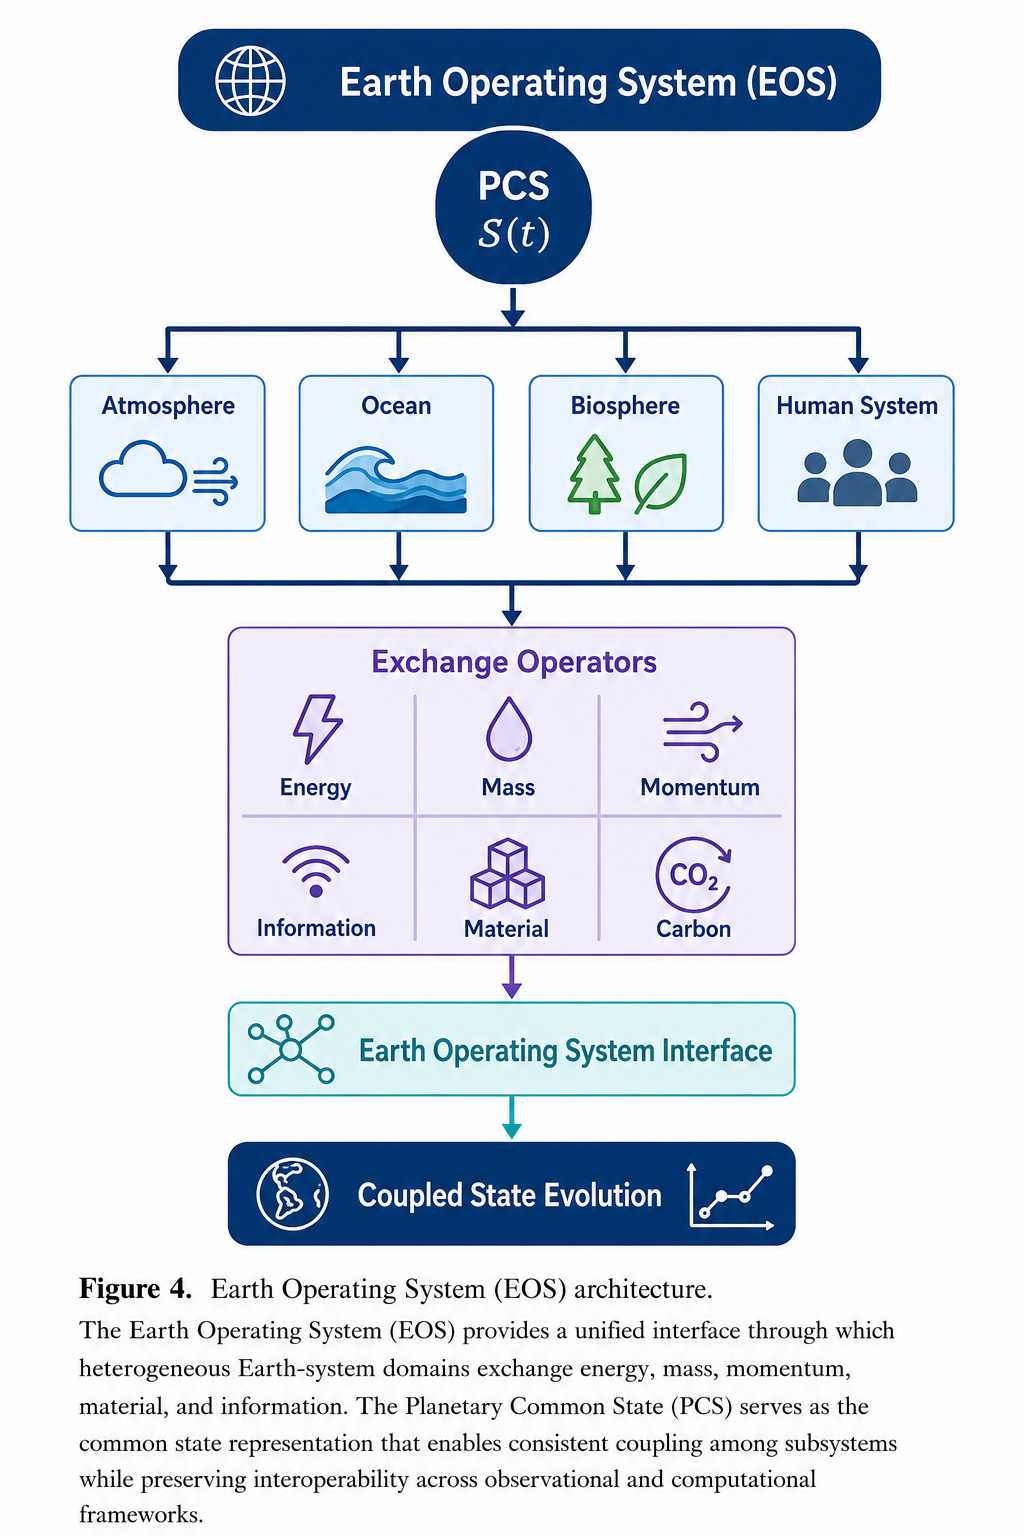
\includegraphics[width=\columnwidth]{figures/fig04_eos_architecture.png}
\caption{Earth Operating System (EOS) architecture.}
\label{fig:fig04_eos_architecture}
\end{figure}

\subsection{9.1 Multi-Source Assimilation}

Observations differ in spatial resolution, temporal sampling, measurement uncertainty, and domain interpretation. A generalized assimilation formulation may therefore estimate \(\hat{\mathbb{L}}\) by minimizing an objective function:

\[ \hat{\mathbb{L}}=\arg\min_{\mathbb{L}} J(\mathbb{L}). \]

\begin{figure}[tb]
\centering
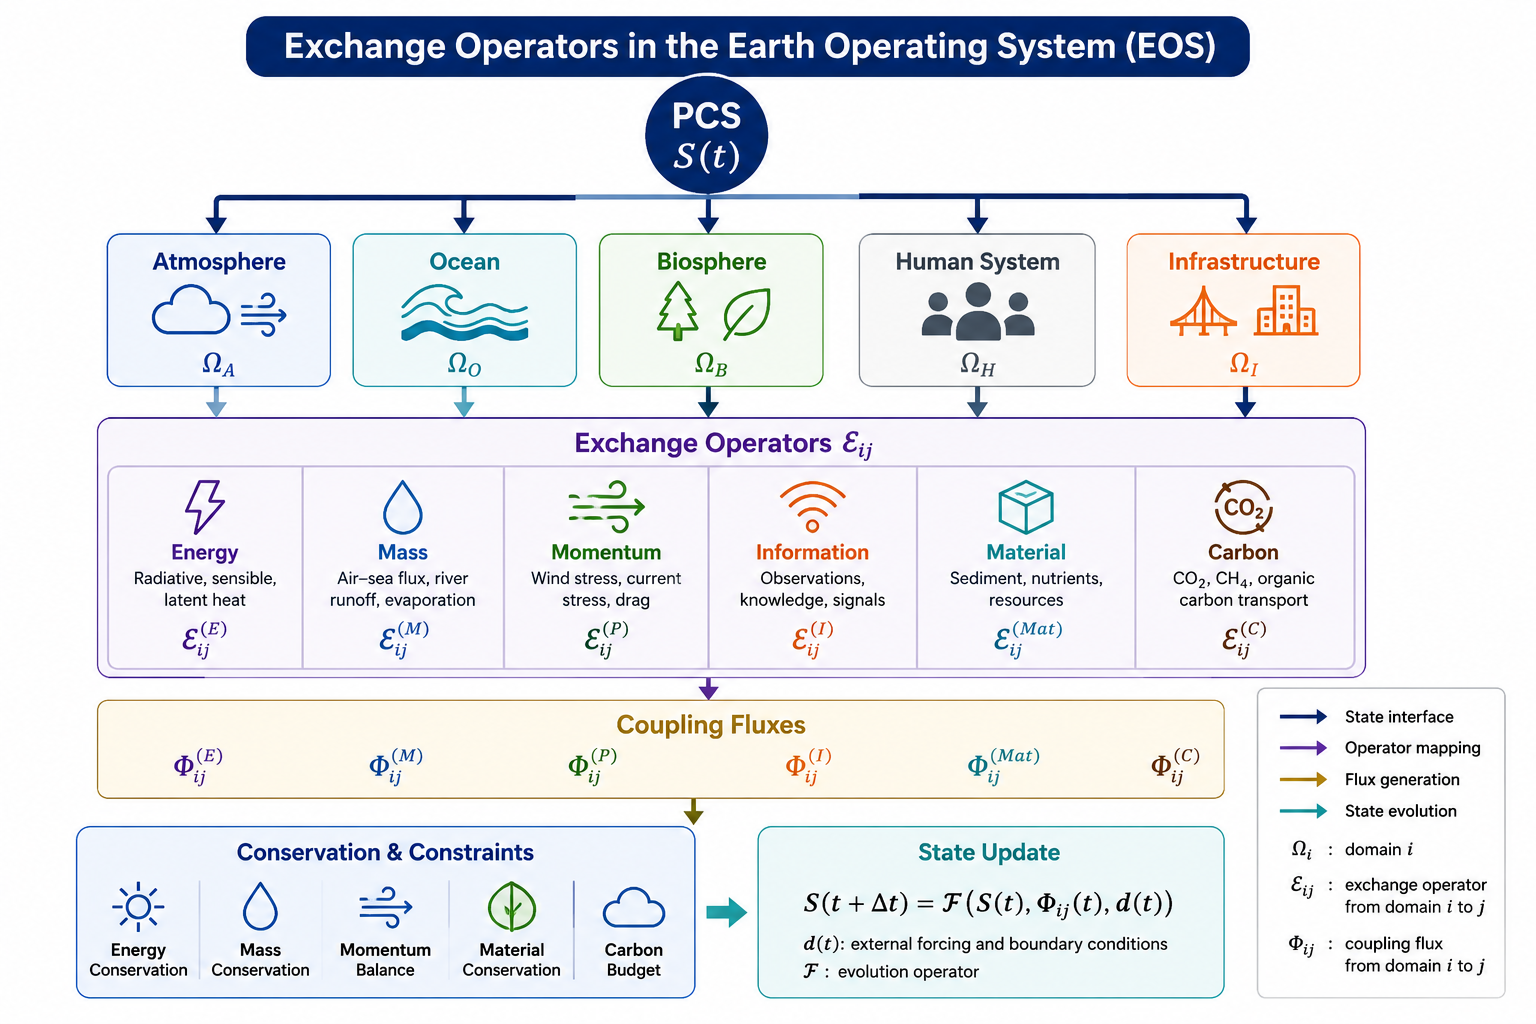
\includegraphics[width=\columnwidth]{figures/fig05_exchange_operators.png}
\caption{Exchange operators in the Earth Operating System (EOS).}
\label{fig:fig05_exchange_operators}
\end{figure}

\subsection{9.2 Cost Function}

A typical cost function may include a background term, an observation term, and a coupling-consistency term:

\[ J=J_b+J_o+J_c. \]

\[ J_c=\|C_{\mathrm{obs}}-C_{\mathrm{model}}\|^2. \]

This term should be used only when the observed and modeled coupling matrices are defined consistently.

\subsection{9.3 Uncertainty}

Uncertainty in the estimated operator may be summarized by

\[ \Sigma_{\mathbb{L}}=\mathrm{Cov}(\hat{\mathbb{L}}). \]

Uncertainty should be propagated through projections, scalar indices, coupling estimates, and hindcasting diagnostics.

\subsection{9.4 Real-Time Updating}

As new observations become available, the estimate may be updated by

\[ \hat{\mathbb{L}}_{k+1}=\mathcal{U}(\hat{\mathbb{L}}_k,\Omega_{k+1}). \]

\(\mathcal{U}\) may be implemented using ensemble filters \cite{Kalnay2003Assimilation}, variational assimilation \cite{Kalnay2003Assimilation}, Bayesian updating \cite{Jaynes1957I}, or other data-assimilation methods \cite{Kalnay2003Assimilation}.

The assimilation equations specify an estimation strategy, not a unique algorithm. The choice of objective function, uncertainty model, and update operator must be justified for each dataset and application.


